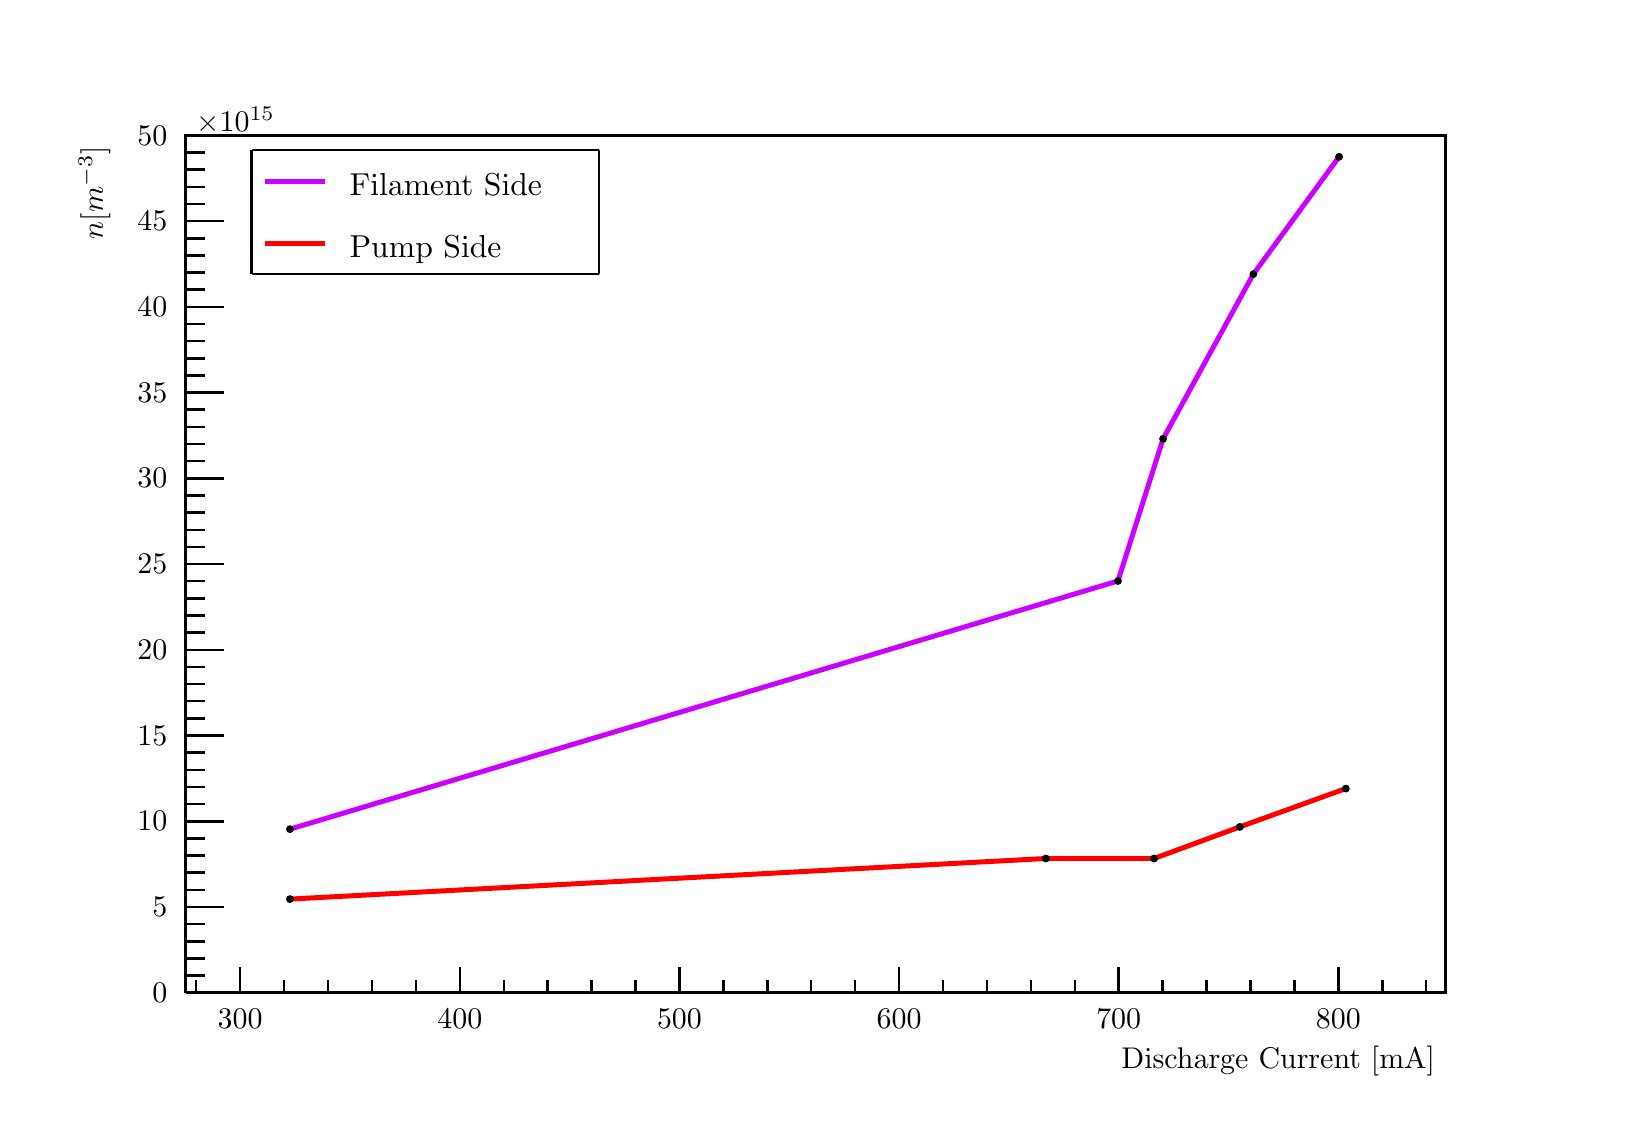
\begin{tikzpicture}
\pgfdeclareplotmark{cross} {
\pgfpathmoveto{\pgfpoint{-0.3\pgfplotmarksize}{\pgfplotmarksize}}
\pgfpathlineto{\pgfpoint{+0.3\pgfplotmarksize}{\pgfplotmarksize}}
\pgfpathlineto{\pgfpoint{+0.3\pgfplotmarksize}{0.3\pgfplotmarksize}}
\pgfpathlineto{\pgfpoint{+1\pgfplotmarksize}{0.3\pgfplotmarksize}}
\pgfpathlineto{\pgfpoint{+1\pgfplotmarksize}{-0.3\pgfplotmarksize}}
\pgfpathlineto{\pgfpoint{+0.3\pgfplotmarksize}{-0.3\pgfplotmarksize}}
\pgfpathlineto{\pgfpoint{+0.3\pgfplotmarksize}{-1.\pgfplotmarksize}}
\pgfpathlineto{\pgfpoint{-0.3\pgfplotmarksize}{-1.\pgfplotmarksize}}
\pgfpathlineto{\pgfpoint{-0.3\pgfplotmarksize}{-0.3\pgfplotmarksize}}
\pgfpathlineto{\pgfpoint{-1.\pgfplotmarksize}{-0.3\pgfplotmarksize}}
\pgfpathlineto{\pgfpoint{-1.\pgfplotmarksize}{0.3\pgfplotmarksize}}
\pgfpathlineto{\pgfpoint{-0.3\pgfplotmarksize}{0.3\pgfplotmarksize}}
\pgfpathclose
\pgfusepathqstroke
}
\pgfdeclareplotmark{cross*} {
\pgfpathmoveto{\pgfpoint{-0.3\pgfplotmarksize}{\pgfplotmarksize}}
\pgfpathlineto{\pgfpoint{+0.3\pgfplotmarksize}{\pgfplotmarksize}}
\pgfpathlineto{\pgfpoint{+0.3\pgfplotmarksize}{0.3\pgfplotmarksize}}
\pgfpathlineto{\pgfpoint{+1\pgfplotmarksize}{0.3\pgfplotmarksize}}
\pgfpathlineto{\pgfpoint{+1\pgfplotmarksize}{-0.3\pgfplotmarksize}}
\pgfpathlineto{\pgfpoint{+0.3\pgfplotmarksize}{-0.3\pgfplotmarksize}}
\pgfpathlineto{\pgfpoint{+0.3\pgfplotmarksize}{-1.\pgfplotmarksize}}
\pgfpathlineto{\pgfpoint{-0.3\pgfplotmarksize}{-1.\pgfplotmarksize}}
\pgfpathlineto{\pgfpoint{-0.3\pgfplotmarksize}{-0.3\pgfplotmarksize}}
\pgfpathlineto{\pgfpoint{-1.\pgfplotmarksize}{-0.3\pgfplotmarksize}}
\pgfpathlineto{\pgfpoint{-1.\pgfplotmarksize}{0.3\pgfplotmarksize}}
\pgfpathlineto{\pgfpoint{-0.3\pgfplotmarksize}{0.3\pgfplotmarksize}}
\pgfpathclose
\pgfusepathqfillstroke
}
\pgfdeclareplotmark{newstar} {
\pgfpathmoveto{\pgfqpoint{0pt}{\pgfplotmarksize}}
\pgfpathlineto{\pgfqpointpolar{44}{0.5\pgfplotmarksize}}
\pgfpathlineto{\pgfqpointpolar{18}{\pgfplotmarksize}}
\pgfpathlineto{\pgfqpointpolar{-20}{0.5\pgfplotmarksize}}
\pgfpathlineto{\pgfqpointpolar{-54}{\pgfplotmarksize}}
\pgfpathlineto{\pgfqpointpolar{-90}{0.5\pgfplotmarksize}}
\pgfpathlineto{\pgfqpointpolar{234}{\pgfplotmarksize}}
\pgfpathlineto{\pgfqpointpolar{198}{0.5\pgfplotmarksize}}
\pgfpathlineto{\pgfqpointpolar{162}{\pgfplotmarksize}}
\pgfpathlineto{\pgfqpointpolar{134}{0.5\pgfplotmarksize}}
\pgfpathclose
\pgfusepathqstroke
}
\pgfdeclareplotmark{newstar*} {
\pgfpathmoveto{\pgfqpoint{0pt}{\pgfplotmarksize}}
\pgfpathlineto{\pgfqpointpolar{44}{0.5\pgfplotmarksize}}
\pgfpathlineto{\pgfqpointpolar{18}{\pgfplotmarksize}}
\pgfpathlineto{\pgfqpointpolar{-20}{0.5\pgfplotmarksize}}
\pgfpathlineto{\pgfqpointpolar{-54}{\pgfplotmarksize}}
\pgfpathlineto{\pgfqpointpolar{-90}{0.5\pgfplotmarksize}}
\pgfpathlineto{\pgfqpointpolar{234}{\pgfplotmarksize}}
\pgfpathlineto{\pgfqpointpolar{198}{0.5\pgfplotmarksize}}
\pgfpathlineto{\pgfqpointpolar{162}{\pgfplotmarksize}}
\pgfpathlineto{\pgfqpointpolar{134}{0.5\pgfplotmarksize}}
\pgfpathclose
\pgfusepathqfillstroke
}
\definecolor{c}{rgb}{1,1,1};
\draw [color=c, fill=c] (0,0) rectangle (20,13.6103);
\draw [color=c, fill=c] (2,1.36103) rectangle (18,12.2493);
\definecolor{c}{rgb}{0,0,0};
\draw [c,line width=0.9] (2,1.36103) -- (2,12.2493) -- (18,12.2493) -- (18,1.36103) -- (2,1.36103);
\definecolor{c}{rgb}{1,1,1};
\draw [color=c, fill=c] (2,1.36103) rectangle (18,12.2493);
\definecolor{c}{rgb}{0,0,0};
\draw [c,line width=0.9] (2,1.36103) -- (2,12.2493) -- (18,12.2493) -- (18,1.36103) -- (2,1.36103);
\draw [c,line width=0.9] (2,1.36103) -- (18,1.36103);
\draw [c,line width=0.9] (2.69177,1.68768) -- (2.69177,1.36103);
\draw [c,line width=0.9] (3.24965,1.52436) -- (3.24965,1.36103);
\draw [c,line width=0.9] (3.80753,1.52436) -- (3.80753,1.36103);
\draw [c,line width=0.9] (4.36541,1.52436) -- (4.36541,1.36103);
\draw [c,line width=0.9] (4.92329,1.52436) -- (4.92329,1.36103);
\draw [c,line width=0.9] (5.48117,1.68768) -- (5.48117,1.36103);
\draw [c,line width=0.9] (6.03905,1.52436) -- (6.03905,1.36103);
\draw [c,line width=0.9] (6.59693,1.52436) -- (6.59693,1.36103);
\draw [c,line width=0.9] (7.15481,1.52436) -- (7.15481,1.36103);
\draw [c,line width=0.9] (7.71269,1.52436) -- (7.71269,1.36103);
\draw [c,line width=0.9] (8.27057,1.68768) -- (8.27057,1.36103);
\draw [c,line width=0.9] (8.82845,1.52436) -- (8.82845,1.36103);
\draw [c,line width=0.9] (9.38633,1.52436) -- (9.38633,1.36103);
\draw [c,line width=0.9] (9.94421,1.52436) -- (9.94421,1.36103);
\draw [c,line width=0.9] (10.5021,1.52436) -- (10.5021,1.36103);
\draw [c,line width=0.9] (11.06,1.68768) -- (11.06,1.36103);
\draw [c,line width=0.9] (11.6179,1.52436) -- (11.6179,1.36103);
\draw [c,line width=0.9] (12.1757,1.52436) -- (12.1757,1.36103);
\draw [c,line width=0.9] (12.7336,1.52436) -- (12.7336,1.36103);
\draw [c,line width=0.9] (13.2915,1.52436) -- (13.2915,1.36103);
\draw [c,line width=0.9] (13.8494,1.68768) -- (13.8494,1.36103);
\draw [c,line width=0.9] (14.4073,1.52436) -- (14.4073,1.36103);
\draw [c,line width=0.9] (14.9651,1.52436) -- (14.9651,1.36103);
\draw [c,line width=0.9] (15.523,1.52436) -- (15.523,1.36103);
\draw [c,line width=0.9] (16.0809,1.52436) -- (16.0809,1.36103);
\draw [c,line width=0.9] (16.6388,1.68768) -- (16.6388,1.36103);
\draw [c,line width=0.9] (2.69177,1.68768) -- (2.69177,1.36103);
\draw [c,line width=0.9] (2.13389,1.52436) -- (2.13389,1.36103);
\draw [c,line width=0.9] (16.6388,1.68768) -- (16.6388,1.36103);
\draw [c,line width=0.9] (17.1967,1.52436) -- (17.1967,1.36103);
\draw [c,line width=0.9] (17.7545,1.52436) -- (17.7545,1.36103);
\draw [anchor=base] (2.69177,0.911891) node[scale=1.08185, color=c, rotate=0]{300};
\draw [anchor=base] (5.48117,0.911891) node[scale=1.08185, color=c, rotate=0]{400};
\draw [anchor=base] (8.27057,0.911891) node[scale=1.08185, color=c, rotate=0]{500};
\draw [anchor=base] (11.06,0.911891) node[scale=1.08185, color=c, rotate=0]{600};
\draw [anchor=base] (13.8494,0.911891) node[scale=1.08185, color=c, rotate=0]{700};
\draw [anchor=base] (16.6388,0.911891) node[scale=1.08185, color=c, rotate=0]{800};
\draw [anchor= east] (18,0.499771) node[scale=1.08185, color=c, rotate=0]{Discharge Current [mA]};
\draw [c,line width=0.9] (2,1.36103) -- (2,12.2493);
\draw [c,line width=0.9] (2.48,1.36103) -- (2,1.36103);
\draw [c,line width=0.9] (2.24,1.5788) -- (2,1.5788);
\draw [c,line width=0.9] (2.24,1.79656) -- (2,1.79656);
\draw [c,line width=0.9] (2.24,2.01433) -- (2,2.01433);
\draw [c,line width=0.9] (2.24,2.23209) -- (2,2.23209);
\draw [c,line width=0.9] (2.48,2.44986) -- (2,2.44986);
\draw [c,line width=0.9] (2.24,2.66762) -- (2,2.66762);
\draw [c,line width=0.9] (2.24,2.88539) -- (2,2.88539);
\draw [c,line width=0.9] (2.24,3.10315) -- (2,3.10315);
\draw [c,line width=0.9] (2.24,3.32092) -- (2,3.32092);
\draw [c,line width=0.9] (2.48,3.53868) -- (2,3.53868);
\draw [c,line width=0.9] (2.24,3.75645) -- (2,3.75645);
\draw [c,line width=0.9] (2.24,3.97421) -- (2,3.97421);
\draw [c,line width=0.9] (2.24,4.19198) -- (2,4.19198);
\draw [c,line width=0.9] (2.24,4.40974) -- (2,4.40974);
\draw [c,line width=0.9] (2.48,4.62751) -- (2,4.62751);
\draw [c,line width=0.9] (2.24,4.84527) -- (2,4.84527);
\draw [c,line width=0.9] (2.24,5.06304) -- (2,5.06304);
\draw [c,line width=0.9] (2.24,5.2808) -- (2,5.2808);
\draw [c,line width=0.9] (2.24,5.49857) -- (2,5.49857);
\draw [c,line width=0.9] (2.48,5.71633) -- (2,5.71633);
\draw [c,line width=0.9] (2.24,5.9341) -- (2,5.9341);
\draw [c,line width=0.9] (2.24,6.15186) -- (2,6.15186);
\draw [c,line width=0.9] (2.24,6.36963) -- (2,6.36963);
\draw [c,line width=0.9] (2.24,6.58739) -- (2,6.58739);
\draw [c,line width=0.9] (2.48,6.80516) -- (2,6.80516);
\draw [c,line width=0.9] (2.24,7.02292) -- (2,7.02292);
\draw [c,line width=0.9] (2.24,7.24069) -- (2,7.24069);
\draw [c,line width=0.9] (2.24,7.45845) -- (2,7.45845);
\draw [c,line width=0.9] (2.24,7.67622) -- (2,7.67622);
\draw [c,line width=0.9] (2.48,7.89398) -- (2,7.89398);
\draw [c,line width=0.9] (2.24,8.11175) -- (2,8.11175);
\draw [c,line width=0.9] (2.24,8.32951) -- (2,8.32951);
\draw [c,line width=0.9] (2.24,8.54728) -- (2,8.54728);
\draw [c,line width=0.9] (2.24,8.76504) -- (2,8.76504);
\draw [c,line width=0.9] (2.48,8.98281) -- (2,8.98281);
\draw [c,line width=0.9] (2.24,9.20057) -- (2,9.20057);
\draw [c,line width=0.9] (2.24,9.41834) -- (2,9.41834);
\draw [c,line width=0.9] (2.24,9.6361) -- (2,9.6361);
\draw [c,line width=0.9] (2.24,9.85387) -- (2,9.85387);
\draw [c,line width=0.9] (2.48,10.0716) -- (2,10.0716);
\draw [c,line width=0.9] (2.24,10.2894) -- (2,10.2894);
\draw [c,line width=0.9] (2.24,10.5072) -- (2,10.5072);
\draw [c,line width=0.9] (2.24,10.7249) -- (2,10.7249);
\draw [c,line width=0.9] (2.24,10.9427) -- (2,10.9427);
\draw [c,line width=0.9] (2.48,11.1605) -- (2,11.1605);
\draw [c,line width=0.9] (2.24,11.3782) -- (2,11.3782);
\draw [c,line width=0.9] (2.24,11.596) -- (2,11.596);
\draw [c,line width=0.9] (2.24,11.8138) -- (2,11.8138);
\draw [c,line width=0.9] (2.24,12.0315) -- (2,12.0315);
\draw [c,line width=0.9] (2.48,12.2493) -- (2,12.2493);
\draw [anchor= east] (1.9,1.36103) node[scale=1.08185, color=c, rotate=0]{0};
\draw [anchor= east] (1.9,2.44986) node[scale=1.08185, color=c, rotate=0]{5};
\draw [anchor= east] (1.9,3.53868) node[scale=1.08185, color=c, rotate=0]{10};
\draw [anchor= east] (1.9,4.62751) node[scale=1.08185, color=c, rotate=0]{15};
\draw [anchor= east] (1.9,5.71633) node[scale=1.08185, color=c, rotate=0]{20};
\draw [anchor= east] (1.9,6.80516) node[scale=1.08185, color=c, rotate=0]{25};
\draw [anchor= east] (1.9,7.89398) node[scale=1.08185, color=c, rotate=0]{30};
\draw [anchor= east] (1.9,8.98281) node[scale=1.08185, color=c, rotate=0]{35};
\draw [anchor= east] (1.9,10.0716) node[scale=1.08185, color=c, rotate=0]{40};
\draw [anchor= east] (1.9,11.1605) node[scale=1.08185, color=c, rotate=0]{45};
\draw [anchor= east] (1.9,12.2493) node[scale=1.08185, color=c, rotate=0]{50};
\draw [anchor=base west] (2,12.2969) node[scale=1.08185, color=c, rotate=0]{$\times10^{15}$};
\draw [anchor= east] (0.841547,12.2493) node[scale=1.08185, color=c, rotate=90]{$n [\si{m^{-3}}]$};
\definecolor{c}{rgb}{0.8,0,1};
\draw [c,line width=1.8] (3.32378,3.4384) -- (13.8395,6.59026) -- (14.4126,8.39542) -- (15.5587,10.4871) -- (16.6476,11.9771);
\definecolor{c}{rgb}{0,0,0};
\foreach \P in {(3.32378,3.4384), (13.8395,6.59026), (14.4126,8.39542), (15.5587,10.4871), (16.6476,11.9771)}{\draw[mark options={color=c,fill=c},mark size=1.201201pt,mark=*] plot coordinates {\P};}
\definecolor{c}{rgb}{1,0,0};
\draw [c,line width=1.8] (3.32378,2.55014) -- (12.9226,3.0659) -- (14.298,3.0659) -- (15.3868,3.46705) -- (16.7335,3.95415);
\definecolor{c}{rgb}{0,0,0};
\foreach \P in {(3.32378,2.55014), (12.9226,3.0659), (14.298,3.0659), (15.3868,3.46705), (16.7335,3.95415)}{\draw[mark options={color=c,fill=c},mark size=1.201201pt,mark=*] plot coordinates {\P};}
\definecolor{c}{rgb}{1,1,1};
\draw [color=c, fill=c] (2.83668,10.4871) rectangle (7.24928,12.063);
\definecolor{c}{rgb}{0,0,0};
\draw [c,line width=0.9] (2.83668,10.4871) -- (7.24928,10.4871);
\draw [c,line width=0.9] (7.24928,10.4871) -- (7.24928,12.063);
\draw [c,line width=0.9] (7.24928,12.063) -- (2.83668,12.063);
\draw [c,line width=0.9] (2.83668,12.063) -- (2.83668,10.4871);
\draw [anchor=base west] (3.93983,11.4918) node[scale=1.14549, color=c, rotate=0]{Filament Side};
\definecolor{c}{rgb}{0.8,0,1};
\draw [c,line width=1.8] (3.00215,11.6691) -- (3.77436,11.6691);
\definecolor{c}{rgb}{0,0,0};
\draw [anchor=base west] (3.93983,10.7038) node[scale=1.14549, color=c, rotate=0]{Pump Side};
\definecolor{c}{rgb}{1,0,0};
\draw [c,line width=1.8] (3.00215,10.8811) -- (3.77436,10.8811);
\end{tikzpicture}
